\begin{table*}[t]
\centering
% \captionsetup{justification=centering}
\resizebox{0.99\linewidth}{!}{
\renewcommand\arraystretch{1.1}
\begin{tabular}{@{}lccccccccccccccccc@{}}
\toprule
\multirow{2}{*}{Model} & \multirow{2}{*}{Model Size} & \multicolumn{3}{c}{\textbf{\texttt{Mine Blocks}}} &  & \multicolumn{3}{c}{\textbf{\texttt{Kill Entities}}} &  & \multicolumn{4}{c}{\textbf{\texttt{Craft Items}}} &  & \multicolumn{3}{c}{\textbf{\texttt{Smelt Items}}} \\ \cmidrule(lr){3-5} \cmidrule(lr){7-9} \cmidrule(lr){11-14} \cmidrule(l){16-18} 
 &  & 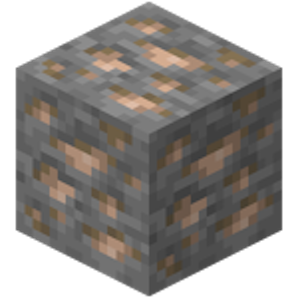
\includegraphics[scale=0.045,valign=c]{figures/avatar/iron_ore.png} & 
\includegraphics[scale=0.035,valign=c]{figures/avatar/obsidian.png} & Avg. &  & 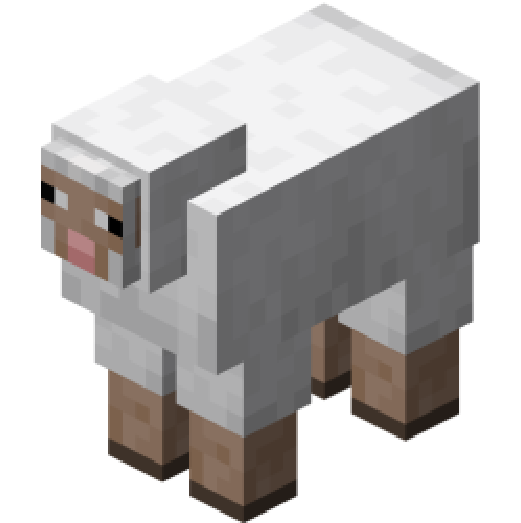
\includegraphics[scale=0.05,valign=c]{figures/avatar/sheep.pdf} & 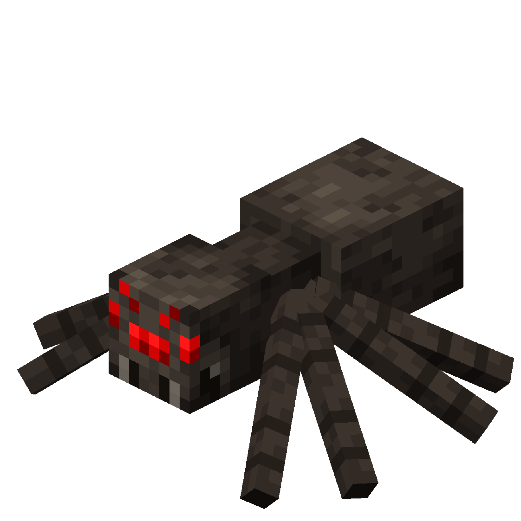
\includegraphics[scale=0.055,valign=c]{figures/avatar/spider.pdf} & Avg. &  & 
\includegraphics[scale=0.08,valign=c]{figures/avatar/crafting_table.png} & 
\includegraphics[scale=0.07,valign=c]{figures/avatar/diamond_sword.png} & 
\includegraphics[scale=0.07,valign=c]{figures/avatar/ladder.png} & Avg. &  & 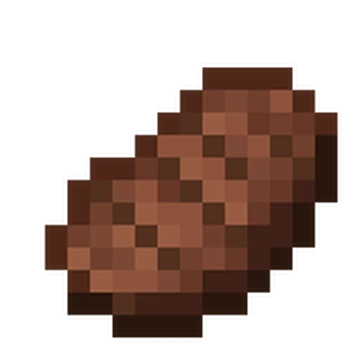
\includegraphics[scale=0.04,valign=c]{figures/avatar/cooked_beef.png} & 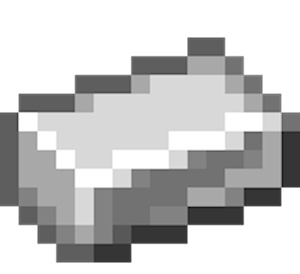
\includegraphics[scale=0.04,valign=c]{figures/avatar/iron_ingot1.jpg} & Avg. \\ \midrule
VPT-BC~\citep{vpt} & 248M & 0.15 & 0.38 & 0.33 &  & \color{blue}{{0.55}} & 0.35 & 0.44 &  & 0.30 & \color{blue}{{0.50}} & 0.45 & 0.41 &  & 0.10 & 0.00 & 0.05 \\
VPT-RL~\citep{vpt} & 248M & 0.05 & 0.35 & 0.25 &  & 0.35 & 0.25 & 0.28 &  & \color{blue}{{0.50}} & 0.30 & 0.62 & 0.55 &  & 0.05 & 0.35 & 0.20 \\
STEVE-1~\citep{steve1} & 248M & 0.20 & 0.35 & 0.54 &  & 0.30 & \color{blue}{{0.75}} & 0.38 &  & 0.45 & 0.20 & \color{blue}{{0.70}} & \color{blue}{{0.57}} &  & 0.25 & \color{blue}{{0.40}} & \color{blue}{{0.33}} \\
GROOT~\citep{groot} & 248M & \color{blue}{{0.56}} & \color{blue}{{0.40}} & \color{blue}{{0.67}} &  & 0.50 & 0.50 & \color{blue}{{0.52}} &  & 0.45 & 0.35 & 0.25 & 0.40 &  & \color{blue}{{0.35}} & 0.25 & 0.30 \\ 
MineDreamer~\citep{minedreamer} & 7B & 0.25 & \color{blue}{{0.40}} & 0.55 &  & 0.30 & 0.70 & 0.39 &  & \color{blue}{{0.50}} & 0.25 & 0.30 & 0.42 &  & 0.30 & 0.30 & 0.30 \\ \midrule
Qwen2-VL~(raw) & 7B & 0.77 & 0.60 & 0.79 &  & 0.93 & 0.80 & 0.84 &  & 0.83 & 0.53 & 0.40 & 0.60 &  & 0.03 & 0.10 & 0.07 \\
Qwen2-VL~(IL) & 7B & 0.70 & 0.73 &  0.75 & & 0.97 & 0.83 & 0.86 & & 0.73 & 0.67 & 0.50 &  0.65 & & 0.17 & 0.37 & 0.29 \\
\model-Qwen2 & 7B & \color{red}{\textbf{0.80}} & \color{red}{\textbf{0.95}} & \color{red}{\textbf{0.88}} &  & \color{red}{\textbf{0.97}} & \color{red}{\textbf{0.93}} & \color{red}{\textbf{0.95}} &  & \color{red}{\textbf{0.87}} & \color{red}{\textbf{0.83}} & \color{red}{\textbf{0.63}} & \color{red}{\textbf{0.77}} &  & \color{red}{\textbf{0.77}} & \color{red}{\textbf{0.70}} & \color{red}{\textbf{0.70}} \\ \bottomrule
\end{tabular}}
\caption{
Evaluation results of different policies on Minecraft tasks, %categorized into Mine Blocks, Kill Entities, Craft Items, and Smelt Items. 
Each group includes multiple tasks (at least 5), and the Avg. column reports the average success rate within each group. Qwen2-VL, Qwen2-VL~(IL) and \model-Qwen2-VL represent the training on the original qwen checkpoint, post-training on only large-scale imitation learning trajectories, and post-trained on VLP intermediate model. Qwen2-VL~(\method) achieves the highest success rates across all task groups. 
}
\label{tab:atom_tasks}
\end{table*}